% !TEX root = ../document.tex
\section{Blockchain in der Theorie}
\label{sec:Theorie}
Die Blockchain ist eine verkette Liste von Blöcken, welche mithilfe von kryptographischen Verfahren irreversible und manipulationsfrei verbunden sind. Ein Block enthält Transaktionen in denen Daten gespeichert sind. Eine Blockchain besteht nicht aus einer zentralen Datenbank, sondern wird in einem dezentralen Peer-To-Peer Netzwerk gespeichert. In einem Peer-To-Peer Netzwerk werden die Netzwerkteilnehmer als Nodes bezeichnet.\footnote{\cite[S.~5]{Korzun.2013}}


\subsection{Transaktionsablauf}
\label{subsec:transaktionsablauf}
Eine Transaktion ist eine Arbeitseinheit, welche eine bestimmte Funktion erf{\"u}llt. In Bezug auf Datenbanksysteme bezeichnet eine Transaktion eine Folge von Datenverarbeitungsbefehlen, die vom System atomar ausgef{\"u}hrt werden.\footnote{\cite[S.~301]{Kemper.2006}} Im Kontext der Blockchain bezeichnet eine Transaktion die Persistierung von Daten, wie beispielsweise einer {\"U}berweisung von Person a zu Person b.\footnote{\cite[S.~2]{SatoshiNakamoto.}} Abbildung \ref{fig:transaktionsablauf} beschreibt den einfachen Transaktionsablauf einer Blockchain.

\begin{figure}[h]
	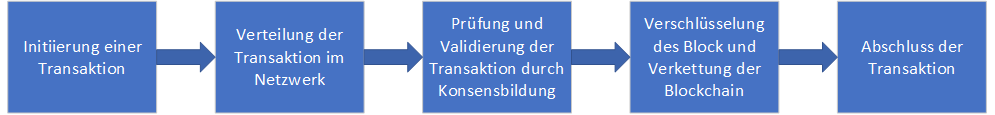
\includegraphics[width=\textwidth]{transaktions-ablauf.png}
	\caption{Vereinfachter Transaktionsablauf. Quelle: Fraunhofer FIT}
	\label{fig:transaktionsablauf}
\end{figure}

Zunächst wird die durchzuführende Transaktion im Netzwerk verteilt. Anschließend fassen die Netzwerkteilnehmer mehrere Transaktionen zu einem Block zusammen und versuchen durch eine Konsensbildung die Transaktionen zu validieren. Die Validierung findet bei der Blockchain-Technologie mit dem sogenannten Proof-Of-Work statt, welche es fordert das aus den Transaktionen und dem vorherigen Block ein Hash mit einer bestimmten Voraussetzung gebildet wird (beispielsweise zehn führende Nullen). Nachdem ein Netzwerkteilnehmer ein validen Hash ermittelt hat, werden der Block an die Kette angehangen und im Netzwerk verteilt. Alle anderen Teilnehmer überprüfen die Erweiterung der Kette. Falls die neue Blockchain nicht den Ansprüchen der Voraussetzung entspricht, wird die Erweiterung abgelehnt und die vorherige Kette zurückgegeben, andernfalls wird die erweiterte Blockchain übernommen. Anschließend ist die Transaktion erfolgreich durchgeführt.


\subsection{Blockaufbau}
\label{subsec:blockaufbau}
Grundsätzlich besteht ein Block einer Blockchain aus den Transaktionen und Informationen über den aktuellen Block. Mithilfe der Merkle-Root wird aus den einzelnen Transaktionen ein Hashwert ermittelt, jener anschließend in Kombination mit dem vorherigen Blockhash und der freiwählbaren Nonce den Hash des aktuellen Blockes bildet. Mithilfe dieser Einbindung des vorherigen Hash wird die Kette fest miteinander verbunden.

\begin{figure}[h]
	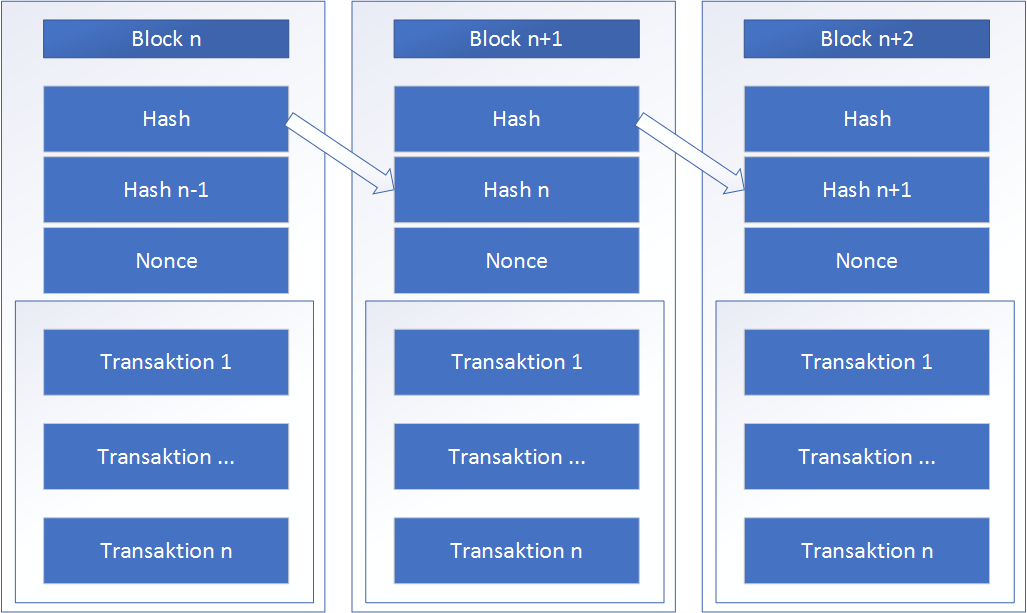
\includegraphics[width=\textwidth]{blockaufbau.png}
	\caption{Blockaufbau. Quelle: Satoshi Nakamoto}
	\label{fig:blockaufbau}
\end{figure}


\subsection{Proof-Of-Work}
\label{subsec:proofofwork}
